\documentclass{article}
\usepackage{graphicx}
\begin{document}
\section{Virtual Topology}
Algorithms are implemented on the tree virtual topology, consisting of five nodes. Each node has an information about its parent in the configuration file. After the cluster is started, nodes connect to their parents establishing the tree topology. Once topology is established, each node holds information about its parent and children.\\
On the picture each circle represents a node, the text inside of the circle being the node's id. Text to the right is node's IP address. Lines show which nodes are connected.\\
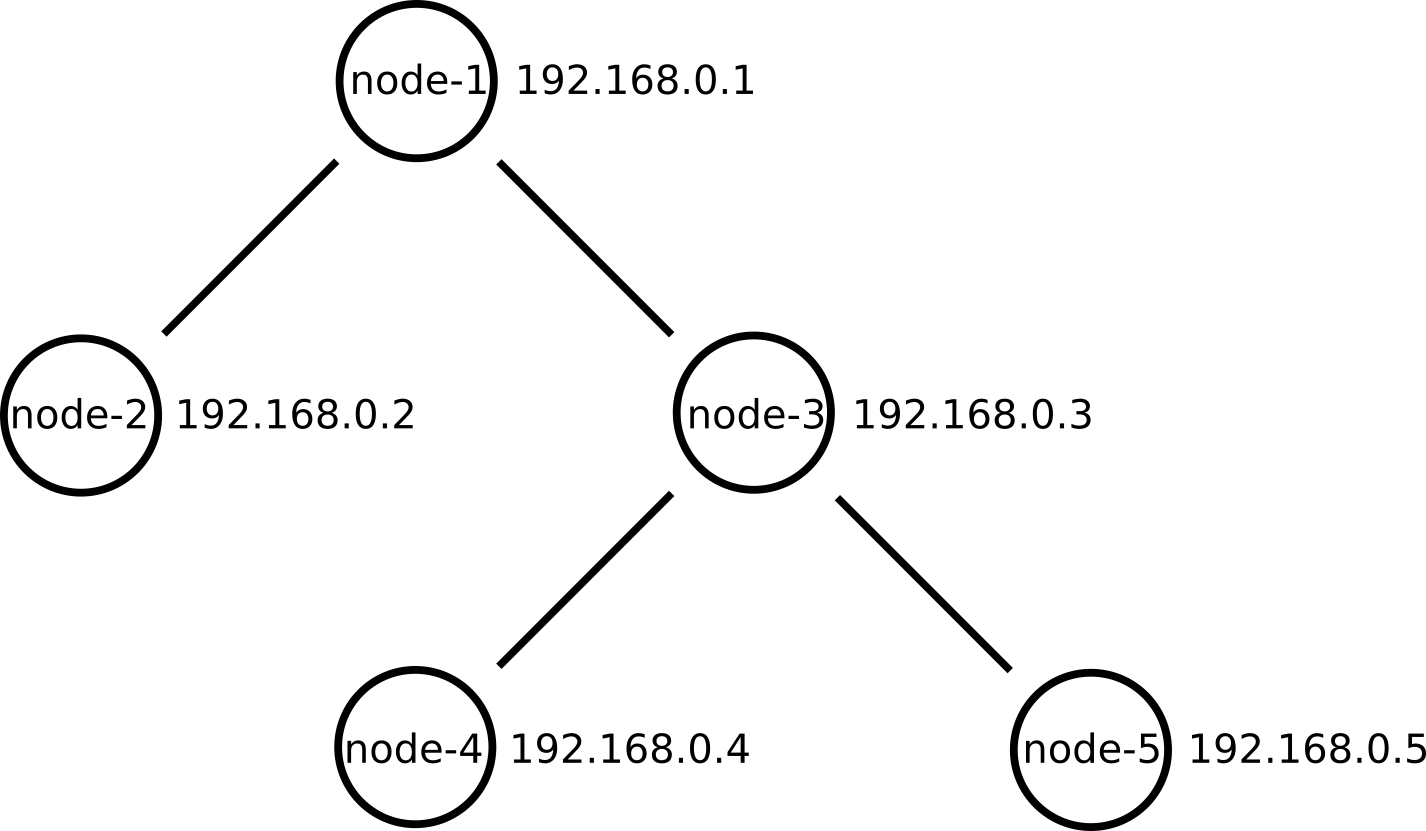
\includegraphics[width=\textwidth]{topology.png}
\section{Leader Election}
Leader election algorithm starts with typing "elect" into the console of any node. Console sends an AssignInitiator message to the corresponding author therefore making it an election initiator. Initiator then sends a BeginElection message to its parent. If it has children, it sends a BeginElection message to each child. If not, it suggests itself as a leader to its parent with ElectionCandidate message.
Each node that received a BeginElection message sends a BeginElection message to everyone it's connected to except the sender of the message. If the node has no children, it suggests itself as a leader to its parent with ElectionCandidate message.\\
When node receives an ElectionCandidate message checks if it got such messages from all its children. If yes, it takes the maximum of the children's and its own ids and sends it to its parent. If it has no parent, it is the tree root, it computes the maximum id and sends it to its children with LeaderElected message.\\
Each node that received a LeaderElection message sends it to everyone it's connected to except the sender. Then the node sends a JoinTeam message to the leader, creating a new virtual topology where every node is connected to the leader (shown in red on the picture).\\
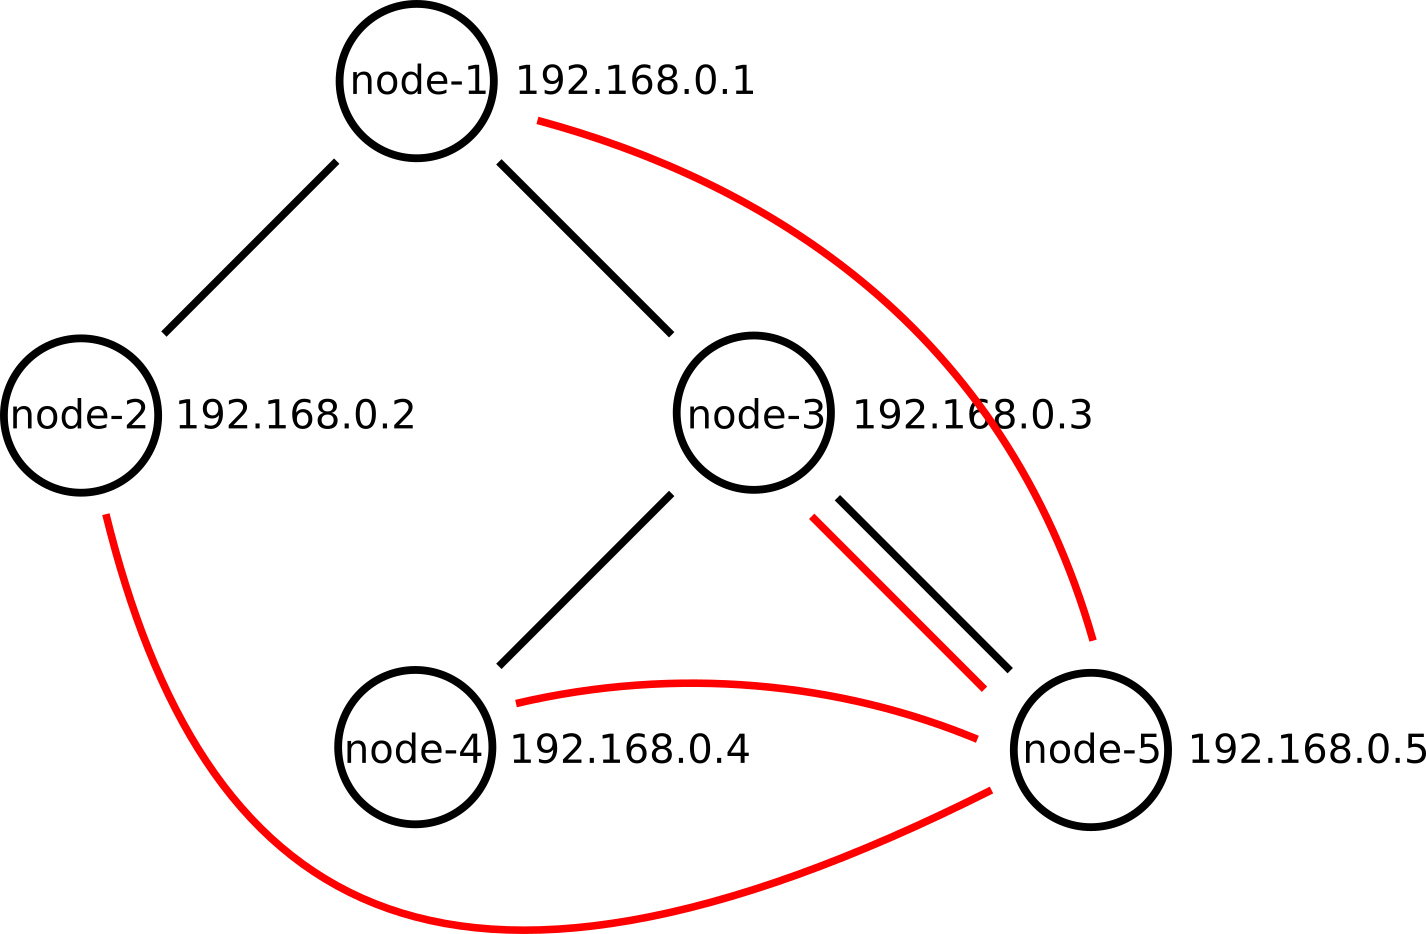
\includegraphics[width=\textwidth]{topology2.png}
\section{Data Collection}
Data collection algorithm starts the same as the leader election algorithm with a kickstart message (CollectData). Node that received it checks if there is a leader and if not, it starts an election.\\
After the leader is elected, the node sends the DataRequest message to the leader.\\
If node that received a DataRequest is the leader, it sends the DataRequest message to all the nodes it is connected to. Otherwise the node sends back a DataChunk message.\\
Once leader receives DataChunk messages from all the connected nodes, it assembles a CompleteData message from them and sends it to the node, requesting the data.
\end{document}
